\documentclass[11pt]{article}
%%
%% Package includes to provide the basic style
%%
\usepackage[top=3.5cm, bottom=3.5cm, left=2.5cm, right=2.5cm]{geometry}
\usepackage{hyperref}
\usepackage{pdfpages}
\usepackage{algorithm2e}
\usepackage[authoryear]{natbib}
\bibliographystyle{plainnat}
\usepackage{appendix}
\usepackage{pgfplotstable}
\usepackage[font={color=darkgray,footnotesize, sf, it}]{caption}
\usepackage{amsmath}
\usepackage{helvet}
\usepackage{wrapfig}
\usepackage{multicol}
\usepackage[eulergreek]{sansmath}
\usepackage{listings}
\usepackage{setspace}
\usepackage{graphicx}
\usepackage{longtable}
\usepackage{minted}
\usepackage{relsize}
\linespread{1.2}
\lstset { %
    language=C++,
    backgroundcolor=\color{black!5}, % set backgroundcolor
    basicstyle=\ttfamily\footnotesize,% basic font setting
}
\usepackage{bchart}
\usepackage{booktabs}
\usepackage{xcolor}

\definecolor{skyblue}{RGB}{203,240,255}
\definecolor{forestgreen}{RGB}{0,96,50}
\definecolor{indigo}{RGB}{4,87,239}
\definecolor{darkindigo}{RGB}{1,40,112}
\definecolor{darkpurple}{RGB}{32,14,104}
\definecolor{apple}{RGB}{0,158,13}
\definecolor{bad}{RGB}{239,55,55}
\definecolor{badtoavg}{RGB}{247,128,98}
\definecolor{avg}{RGB}{255,218,117}
\definecolor{avgtogood}{RGB}{190,247,140}
\definecolor{good}{RGB}{102,226,102}

\setlength{\parindent}{0em}
\setlength{\parskip}{1em}
\setlength\parindent{0pt}

\usepackage{titling}
\usepackage{titlesec}
\pretitle{\Huge\bfseries}
\posttitle{\par}

\titlespacing\section{0pt}{12pt plus 4pt minus 2pt}{0pt plus 2pt minus 2pt}
\titlespacing\subsection{0pt}{12pt plus 4pt minus 2pt}{0pt plus 2pt minus 2pt}
\titlespacing\subsubsection{0pt}{12pt plus 4pt minus 2pt}{0pt plus 2pt minus 2pt}

\usepackage[english]{babel}
\usepackage[utf8]{inputenc}
\usepackage{fancyhdr}
 
\pagestyle{fancy}
\fancyhf{}
\rhead{cjd47}
\lhead{CM30141: \textit{Theory of Human-Computer Interaction}}
\cfoot{\thepage} 
\renewcommand{\headrulewidth}{1pt}
\renewcommand{\footrulewidth}{1pt}

\newcommand\wordcount[1]{
\vfill
\textit{Word count: {#1} words (not inc. Citations, Figures or References)}}

\newcommand\essaytitle[1]{
\begin{LARGE}
\textbf{{#1}} \\
\end{LARGE}}

\newcommand\sectiontitle[1]{
\begin{large}
\textbf{{#1}} \medskip \\ 
\end{large}}

%%
%% END OF DEFINITIONS
%%

\begin{document}
\essaytitle{Critical Review: Exploring Interactions with Physically Dynamic Bar Charts}

\sectiontitle{Introduction}
Studies investigating how data can be effectively presented to, explored and interpreted by users forms the core part of Information Visualisation (`InfoVis') to support users in the decision-making process. This review summarises and critically analyses \citet{taher2015} whose paper explores the use of physically dynamic bar charts as devices for exploring user interactions with visualisations of data, to determine future work in this domain of Information Visualisation.

\sectiontitle{Summary of Contributions}
\citeauthor{taher2015} seeks to extend existing work on use of physical visualisations (\textit{physicalizations}) \citep{jansen2015} to investigate how users interact with \textit{physically dynamic} bar charts as a way of exploring and manipulating shape-changing datasets in the physical world. Much of the existing work reliant on use of physicalizations involve problematic \textit{static} models that do not respond to user interactions \citep{jansen2013} and are therefore ``\textit{disconnected}'' from the source of the data when they are created. With the advent of shape-changing technology and tangible interfaces \citep{rasmussen2012}, there is a window of opportunity for the manufacture of physically dynamic displays to help decision makers reason about and manipulate data sets in a non-virtual and non-static way. It is this motivation that leads \citeauthor{taher2015} to explore the ways users interact with data displayed in this mode to understand whether \textit{physical} interactions with data (such as touching specific bars) or \textit{gestures} (such as swiping a touch-screen) or a combination of the two is more intuitive to users interacting with data visualisations in order to solve common problems. Whilst the authors concede that the use of physical dynamic visualisations is not new \citep{leithinger2010,follmer2013}, they claim there is little in the way of analysis into effective \textit{interactions} with data of \textit{dynamic} physical modality, unlike the abundance of work investigating their static counterparts \citep{stusak2014}.

The point system described by the article to support the author's research is \textit{EMERGE} - a $10\times10$ physical bar chart which uses a set of dynamic self-actuating rods with an RGB display projected onto it (Figure \ref{fig:taher2015-emerge}). An immediate and obvious limitation of using a Bar Chart point system is that any conclusions drawn about its effectiveness in physically-dynamic form cannot be generalised to other types of InfoVis systems, such as Dynamic Histograms, Parallel Coordinates and Theme Rivers. 

\begin{figure}[H]
\centering
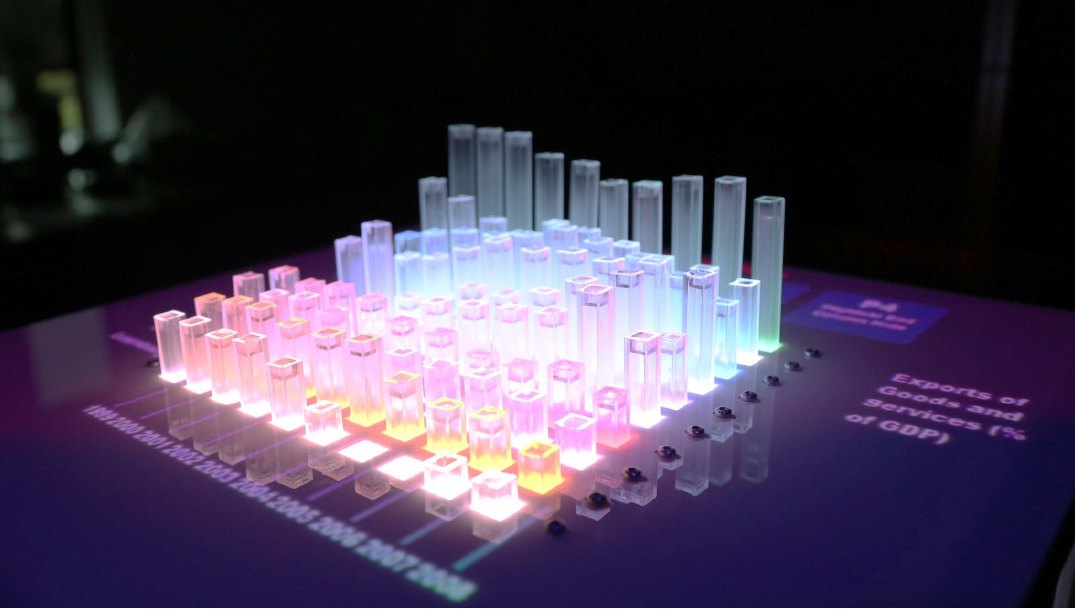
\includegraphics[width=0.5\textwidth]{img/taher2015-emerge.png} 
\caption{EMERGE: Exploring Interactions with Physically Dynamic Bar Charts using actuating physical rods and RGB LEDs to display international export data.}\label{fig:taher2015-emerge}
\end{figure}

EMERGE allows users to interact with the dataset it represents using a set of 4 task-sets derived from subcategories of the taxonomy of interactive dynamics for visual analysis described by \citet{heer2012} - \textit{annotation}, \textit{filtering}, \textit{organisation} and \textit{navigation} (Table \ref{tbl:taher2015-user-study}).  \citeauthor{heer2012} lay out 3 high-level categories in their model - \textit{Data and View Specification}, \textit{View Manipulation}, and \textit{Process and Provenance}. (Figure \ref{fig:heer2012-taxonomy}). In this sense, whilst the selection of InfoVis model is careful and grounded in background theory, the choice of subcategories by \citeauthor{taher2015} for interacting with EMERGE is somewhat arbitrary and limited in scope, which immediately invites further research into different forms of interactions with physicalisations from the taxonomy.

\begin{table}[H]
\centering
\caption{Task-sets and interaction techniques explored during the user study with EMERGE: \textit{annotation}, \textit{filtering}, \textit{organisation} and \textit{navigation} with the category of \protect\citet{heer2012} in \textbf{bold}.}\label{tbl:taher2015-user-study}
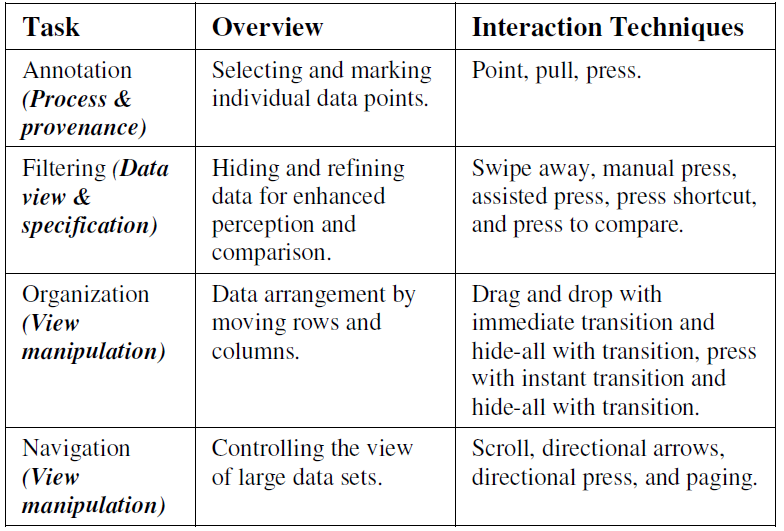
\includegraphics[width=0.65\textwidth]{img/taher2015-user-study.png} 
\end{table}

\begin{figure}[H]
\centering
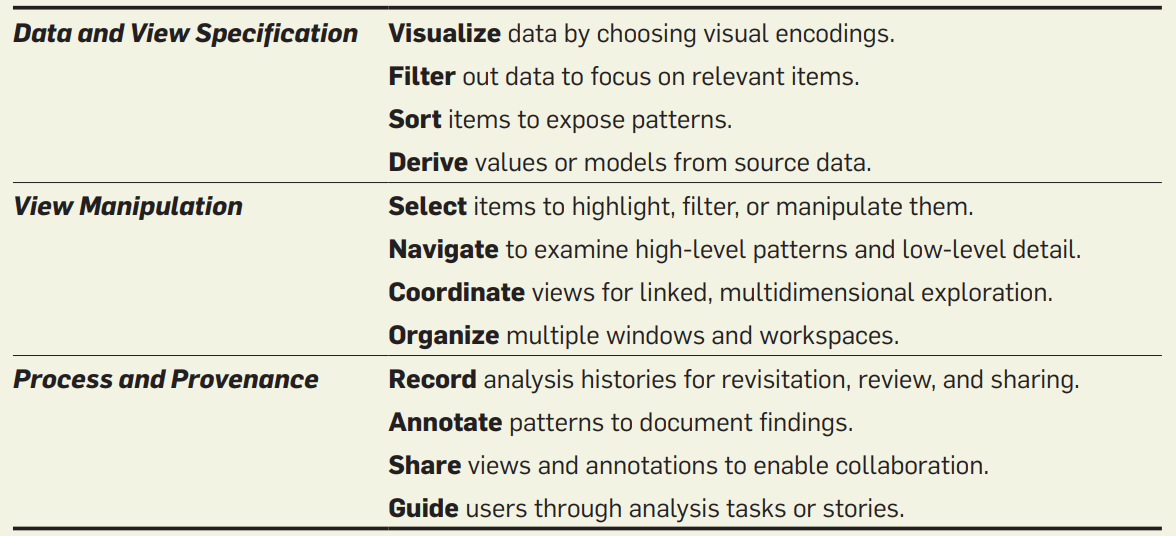
\includegraphics[width=0.8\textwidth]{img/heer2012-taxonomy.png} 
\caption{Taxonomy of interactive dynamics described by \protect\citet{heer2012}.}\label{fig:heer2012-taxonomy}
\end{figure}

The main contributions of \citet{taher2015} is threefold. First, the authors present a set of 14 potential interactions (both physical and gesture based) for manipulating and exploring data presented in dynamic physical bar charts such as EMERGE. Second, the findings of their user study ($N=17$) evaluates which of the 14 interactions are effective and intuitive in completing a set of data analysis tasks, and which interactions match users' initial preconceptions for how to achieve these tasks. Finally, a set of important design considerations are presented to advise future research on the challenges of presenting data in physically dynamic form. Overall, we learn that a combination of gestures and physical interaction is effective. Smaller interactions such as annotation of specific data points can be afforded by physical interaction whereas larger interactions such as organization can be afforded touch-screen gestures. 

\sectiontitle{Justifications for Conclusions}
\citeauthor{taher2015} set about their investigations by creating a list of proposed or \textit{baseline} interactions by which users could interact with EMERGE. The authors by their own admission avoided early experimentation to generate different types of interaction before the main study as existing research forewarned against this due to the immaturity of the area \citep{hornbaek2013}. Whilst this was sensible to consider, the mechanics of the baseline interactions to be used in the user study are strongly-coupled with the hardware capabilities of EMERGE and no explanation is given by the authors into where the inspiration for each proposed interaction came from, which causes some early concern over generalisability of results to other implementations of physically dynamic bar charts.

\begin{figure}[H]
\minipage{0.5\textwidth}
\centering
  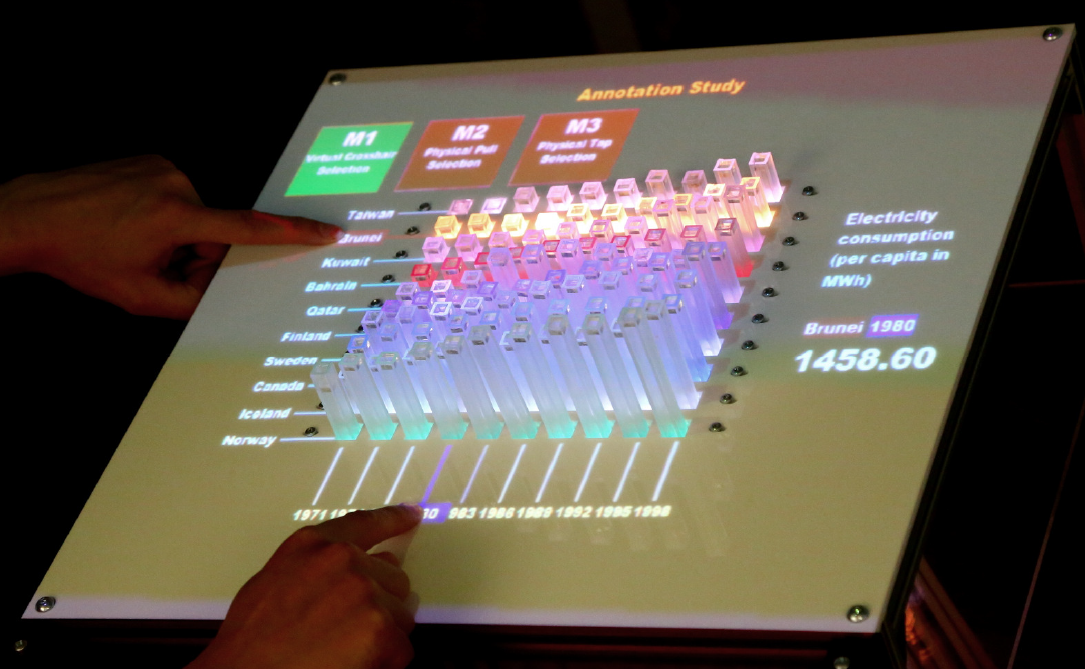
\includegraphics[height=3.5cm]{img/taher2015-annotation.png}
  \caption{Annotation (Point technique).}\label{fig:taher2015-annotation}
\endminipage\hfill
\minipage{0.5\textwidth}%
\centering
  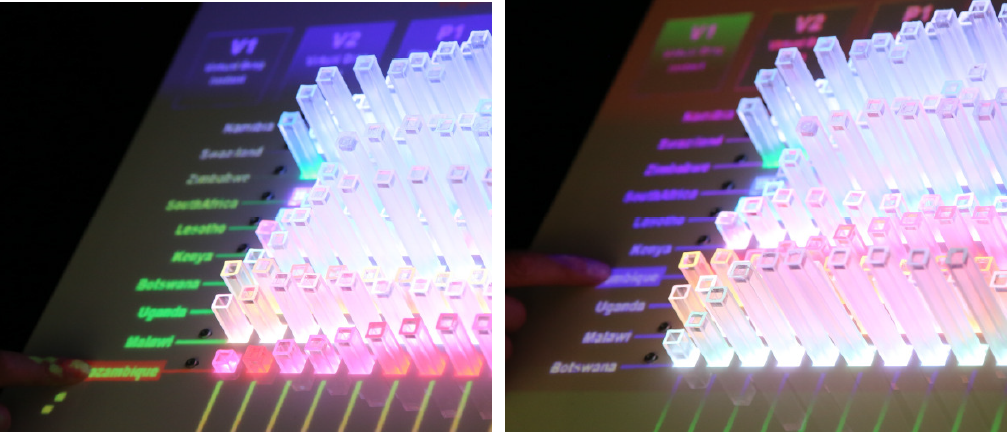
\includegraphics[height=3.5cm]{img/taher2015-organize.png}
  \caption{Organisation (Drag and Drop technique).}\label{fig:taher2015-organize}
\endminipage
\end{figure}

\begin{figure}[H]
\centering
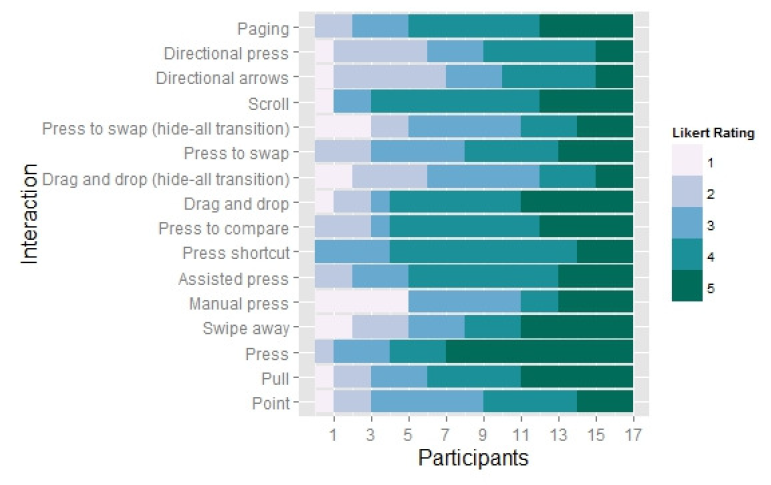
\includegraphics[width=0.5\textwidth]{img/taher2015-likert.png} 
\caption{Likert scale ratings for helpfulness of interaction
techniques. Range = 1: Strongly Disagree, 5: Strongly Agree.}\label{fig:taher2015-likert}
\end{figure}

\sectiontitle{Limitations and Suggested Further Work}
\citet{taher2015} present a respectable overview of potential techniques to interact with data presented in a physically dynamic form, but a set of limitations with their work leads to some questions being open to future research. 

Authors:
\begin{itemize}
\item Data manipulation with external objects
\item Multi-finger input
\item Pressing over time
\item Complex task explorations from taxonomy - undo/redo, different filtering (e.g. thresholding)
\item Combining interactions
\item Controlled studies with performance metrics (e.g. task completion times, accuracy)
\end{itemize}

Novel:
\begin{itemize}
\item Larger datasets - the 10x10 grid limits representations
\item Technical challenges (actuation speed and noise, rod spacing, size of setup) may have mediated the results - no investigation e.g. parallel mediated regression testing into this.
\item Study showed almost all participants hesitant to interact with system due to speed of actuation or noise of actuators
\item Larger sample size - 17 not enough.
\item Excluded vertical axis data - difficult to anticipate how this might change user interactions and behaviours.
\item Not just bar charts!
\item Complex datasets which change in real time - e.g. social networks \citep{federico2011}.
\item Different taxonomy - zoom, select, derive, sort, history.
\item Lack of parametric data - study could investigate performance and accuracy of tasks being completed.
\item Apply it to a specific context to compare across modalities in an educational setting for those who learn best by adopting kinaesthetic techniques \citep{gilakjani2011} or even used in a VR-kin setting \citep{tennent2017}.
\end{itemize}

\sectiontitle{Conclusion}
\citet{taher2015} set the foundations for future investigations into use of shape-changing displays for accomplishment of common InfoVis tasks. Their research is limited in several ways by the implementation of the EMERGE system, but raises important design considerations for future work investigating dynamic physicalisations in other domains. Findings have potentially wider consequences in the topic of Information Visualisation - with recommendations on how to design systems supporting the fundamental interactions such as those described by \citet{heer2012}, these visualisations can serve as effective data analysis tools in a variety of domains.

\wordcount{0}

\newpage
\small
\bibliography{bib2}
\normalsize
\end{document}